\documentclass[12pt, a4paper]{article}

\usepackage[utf8]{inputenc}
% Limit the page margin to only 1 inch.
\usepackage[margin=1in]{geometry}

%Imports biblatex package
\usepackage[
backend=biber,
style=alphabetic
]{biblatex}
\addbibresource{../../algs4e.bib}

% Enables the `align' environment.
\usepackage{amsmath}
% Provides useful environments, such as:
% - \begin{proof} ...\end{proof}
\usepackage{amsthm}
% Enables using \mathbb{}, for example \mathbb{N} for the set of natural numbers.
\usepackage{amssymb}

% Allows using letters in enumerate list environment. Use, for example:
%\begin{enumerate}[label=(\alph*)]
% ...
%\end{enumerate}
\usepackage[inline]{enumitem}

% Enable importing external graphic files and provides useful commannds, like \graphicspath{}
\usepackage{graphicx}
% Images are located in a directory called images in the current directory.
\graphicspath{{./images/}}

% Make links look better by default.
% See: https://tex.stackexchange.com/questions/823/remove-ugly-borders-around-clickable-cross-references-and-hyperlinks
\usepackage[hidelinks]{hyperref}
\usepackage{xcolor}
\hypersetup{
	colorlinks,
	linkcolor={red!50!black},
	citecolor={blue!50!black},
	urlcolor={blue!80!black}
}


% Code Listings. Source:
% https://stackoverflow.com/questions/3175105/inserting-code-in-this-latex-document-with-indentation
\usepackage{listings}
\usepackage{color}

\definecolor{dkgreen}{rgb}{0,0.6,0}
\definecolor{gray}{rgb}{0.5,0.5,0.5}
\definecolor{mauve}{rgb}{0.58,0,0.82}

\lstset{frame=tb,
	language=Java,
	aboveskip=3mm,
	belowskip=3mm,
	showstringspaces=false,
	columns=flexible,
	basicstyle={\small\ttfamily},
	numbers=none,
	numberstyle=\tiny\color{gray},
	keywordstyle=\color{blue},
	commentstyle=\color{dkgreen},
	stringstyle=\color{mauve},
	breaklines=true,
	breakatwhitespace=true,
	tabsize=3
}

\newcommand{\prob}{\text{P}}
%\newcommand{\complement}{\mathsf{c}}

% Define an environment called "ex" (for Exercise) so that I can do: \begin{ex}{1.5}...\end{ex}
\newenvironment{ex}[2][Exercise]
{\par\medskip\noindent \textbf{#1 #2.}}
{\medskip}

% Define a solution environment, similar to ex (exercise) environment.
\newenvironment{sol}[1][Solution]
{\par\medskip\noindent \textbf{#1.} }
{\medskip}

\begin{document}
	\noindent Sergio E. Garcia Tapia \hfill
	
	\noindent \emph{Algorithms} by Sedgewick and Wayne (4th edition) \cite{sedgewick_wayne}\hfill
	
	\noindent October 6th, 2024\hfill 
	\section*{1.5: Case Study: Union-find}
	\begin{ex}{1}
		Show the contents of the \texttt{id[]} array and the number of times the array is
		accessed for each input pair when you use quick-find for the sequence
		\begin{lstlisting}[language={}]
9-0 3-4 5-8 7-2 2-1 5-7 0-3 4-2
		\end{lstlisting}
	\end{ex}
	\begin{sol}
		\begin{center}
			\begin{tabular}{cc|cccccccccc|c}
				\multicolumn{13}{c}{\texttt{id[]} (Quick-Find)}\\
				\texttt{p} & \texttt{q} & 0 & 1 & 2 & 3 & 4 & 5 & 6 & 7 & 8 & 9 & Array Accesses\\
				\hline
				9  & 0  & {\color{green} 0} & 1 & 2 & 3 & 4 & 5 & 6 & 7 & 8 & {\color{green} 9} & {}\\
				{} & {} & 0 & 1 & 2 & 3 & 4 & 5 & 6 & 7 & 8 & {\color{red} 0} & 15\\
				3  & 4  & 0 & 1 & 2 & {\color{green} 3} & {\color{green} 4} & 5 & 6 & 7 & 8 & 0 & {}\\
				{} & {} & 0 & 1 & 2 & {\color{red} 4} & 4 & 5 & 6 & 7 & 8 & 0 & 15\\
				5  & 8  & 0 & 1 & 2 & 4 & 4 & {\color{green} 5} & 6 & 7 & {\color{green} 8} & 0 & {}\\
				{} & {} & 0 & 1 & 2 & 4 & 4 & {\color{red} 8} & 6 & 7 & 8 & 0 & 15\\
				7  & 2  & 0 & 1 & {\color{green} 2} & 4 & 4 & 8 & 6 & {\color{green} 7} & 8 & 0 & {}\\
				{} & {} & 0 & 1 & 2 & 4 & 4 & 8 & 6 & {\color{red} 2} & 8 & 0 & 15\\
				2  & 1  & 0 & {\color{green} 1} & {\color{green} 2} & 4 & 4 & 8 & 6 & 2 & 8 & 0 & {}\\
				{} & {} & 0 & 1 & {\color{red} 1} & 4 & 4 & 8 & 6 & {\color{red} 1} & 8 & 0 & 16\\
				5  & 7  & 0 & 1 & 1 & 4 & 4 & {\color{green} 8} & 6 & {\color{green} 1} & 8 & 0 & {}\\
				{} & {} & 0 & 1 & 1 & 4 & 4 & {\color{red} 1} & 6 & 1 & {\color{red} 1} & 0 & 16\\
				0  & 3  & {\color{green} 0} & 1 & 1 & {\color{green} 4} & 4 & 1 & 6 &  1 & 1 & 0 & {} \\
				{} & {} & {\color{red} 4} & 1 & 1 & 4 & 4 & 1 & 6 &  1 & 1 & {\color{red} 4} & 16\\
				4  & 2  & 4 & 1 & {\color{green} 1} & 4 & {\color{green} 4} & 1 & 6 &  1 & 1 & 4 & \\
				{} & {} & {\color{red} 1} & 1 & 1 & {\color{red} 1} & {\color{red} 1} & 1 & 6 &  1 & 1 & {\color{red} 1} & 18\\
			\end{tabular}
		\end{center}
		Each input sequence incurs the cost of a \texttt{connected()} operation which is two
		calls to \texttt{find()}, and hence 2 arrays accesses. Then in calling \texttt{union()},
		we have two more array accesses since  we call \texttt{find()} twice again. Then,
		we have at least 10 array accesses as we iterate through the \texttt{id} array. Finally,
		we have an extra array access for each identifier matching \texttt{pID}, the identifier
		of the component of the first site given.
	\end{sol}
	\begin{ex}{2}
		Do Exercise 1.5.1, but use quick-union (page 224). In addition, draw the forest of trees
		represented by the \texttt{id[]} array after each input pair is processed.
	\end{ex}
	\begin{sol}
		\begin{center}
			\begin{tabular}{cc|cccccccccc|c}
				\multicolumn{13}{c}{\texttt{id[]} (Quick-Union)}\\
				\texttt{p} & \texttt{q} & 0 & 1 & 2 & 3 & 4 & 5 & 6 & 7 & 8 & 9 & Array Accesses\\
				\hline
				9  & 0  & {\color{green} 0} & 1 & 2 & 3 & 4 & 5 & 6 & 7 & 8 & {\color{green} 9} & {}\\
				{} & {} & 0 & 1 & 2 & 3 & 4 & 5 & 6 & 7 & 8 & {\color{red} 0} & 3\\
				
				3  & 4  & 0 & 1 & 2 & {\color{green} 3} & {\color{green} 4} & 5 & 6 & 7 & 8 & 0 & {}\\
				{} & {} & 0 & 1 & 2 & {\color{red} 4} & 4 & 5 & 6 & 7 & 8 & 0 & 3\\
				
				5  & 8  & 0 & 1 & 2 & 4 & 4 & {\color{green} 5} & 6 & 7 & {\color{green} 8} & 0 & {}\\
				{} & {} & 0 & 1 & 2 & 4 & 4 & {\color{red} 8} & 6 & 7 & 8 & 0 & 3\\
				
				7  & 2  & 0 & 1 & {\color{green} 2} & 4 & 4 & 8 & 6 & {\color{green} 7} & 8 & 0 & {}\\
				{} & {} & 0 & 1 & 2 & 4 & 4 & 8 & 6 & {\color{red} 2} & 8 & 0 & 3\\
				
				2  & 1  & 0 & {\color{green} 1} & {\color{green} 2} & 4 & 4 & 8 & 6 & {\color{green} 2} & 8 & 0 & {}\\
				{} & {} & 0 & 1 & {\color{red} 1} & 4 & 4 & 8 & 6 & 2 & 8 & 0 & 3\\
				
				5  & 7  & 0 & {\color{green} 1} & {\color{green} 1} & 4 & 4 & {\color{green} 8} & 6 & {\color{green} 2} & {\color{green} 8} & 0 & {}\\
				{} & {} & 0 & 1 & 1 & 4 & 4 & 8 & 6 & 2 & {\color{red} 1} & 0 & 9\\
				
				0  & 3  & {\color{green}0} & 1 & 1 & {\color{green} 4} & {\color{green} 4} & 8 & 6 & 2 & 1 & {\color{green} 0} & {}\\
				{} & {} & {\color{red} 4} & 1 & 1 & 4 & 4 & 8 & 6 & 2 & 1 & 0 & 5\\
				
				4  & 2  & {\color{green} 4} & {\color{green} 1} & {\color{green} 1} & {\color{green} 4} & {\color{green} 4} & 8 & 6 & 2 & 1 & {\color{green} 9} & {}\\
				{} & {} & 4 & 1 & 1 & 4 & {\color{red} 1} & 8 & 6 & 2 & 1 & 0 & 5\\
			\end{tabular}
		\end{center}
		See Figure~\ref{ex-02} for the forest of trees representation of \texttt{id[]}.
		\begin{figure}
			\centering
			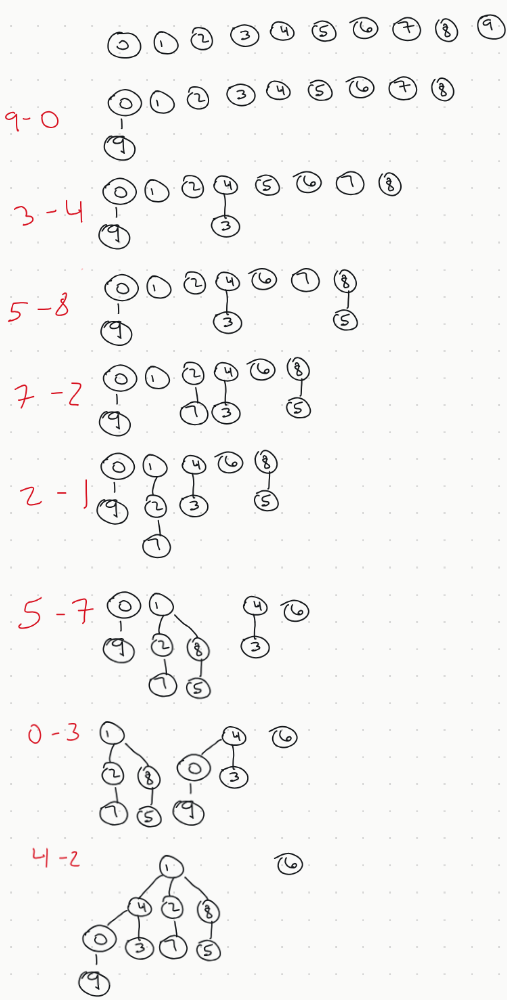
\includegraphics[width=0.5\textwidth]{exercise-02-quick-union-forest-of-trees}
			\caption{Forest of trees representation of \texttt{id[]} for quick-union in Exercise 2.}
			\label{ex-02}
		\end{figure}
	\end{sol}
	\begin{ex}{3}
		Do Exercise 1.5.1, but use weighted quick-union (page 228).
	\end{ex}
	\begin{sol}
		\begin{center}
			\begin{tabular}{cc|cccccccccc|c}
				\multicolumn{13}{c}{\texttt{id[]} Weighted Quick-Union}\\
				\texttt{p} & \texttt{q} & 0 & 1 & 2 & 3 & 4 & 5 & 6 & 7 & 8 & 9 & \texttt{id[]} Array Accesses\\
				\hline
				9  & 0  & {\color{green} 0} & 1 & 2 & 3 & 4 & 5 & 6 & 7 & 8 & {\color{green} 9} & {}\\
				{} & {} & {\color{red} 9} & 1 & 2 & 3 & 4 & 5 & 6 & 7 & 8 & 9 & 3\\
				
				3  & 4  & 9 & 1 & 2 & {\color{green} 3} & {\color{green} 4} & 5 & 6 & 7 & 8 & 9 & {}\\
				{} & {} & 9 & 1 & 2 & 3 & {\color{red} 3} & 5 & 6 & 7 & 8 & 9 & 3\\
				
				5  & 8  & 9 & 1 & 2 & 3 & 3 & {\color{green} 5} & 6 & 7 & {\color{green} 8} & 9 & {}\\
				{} & {} & 9 & 1 & 2 & 3 & 3 & 5 & 6 & 7 & {\color{red} 5} & 9 & 3\\
				
				7  & 2 & 9 & 1 & {\color{green} 2} & 3 & 3 & 5 & 6 & {\color{green} 7} & {\color{red} 5} & 9 & {}\\
				{} & {} & 9 & 1 & {\color{red} 7} & 3 & 3 & 5 & 6 & 7 & {\color{red} 5} & 9 & 3\\
				
				2  & 1 & 9 & {\color{green}1} & {\color{green} 7} & 3 & 3 & 5 & 6 & {\color{green} 7} & 5 & 9 & {}\\
				{} & {} & 9 & {\color{red}7} & 7 & 3 & 3 & 5 & 6 & 7 & 5 & 9 & 5\\
				
				5  & 7 & 9 & {\color{green} 7} & {\color{green} 7} & 3 & 3 & {\color{green} 5} & 6 & {\color{green} 7} & {\color{green}5} & 9 & {}\\
				{} & {} & 9 & 7 & 7 & 3 & 3 & {\color{red} 7} & 6 & {\color{green} 7} & 5 & 9 & 3\\
				
				0  & 3  & {\color{green} 9} & 7 & 7 & {\color{green}3} & {\color{green}3} & 7 & 6 & 7 & 5 & {\color{green}9} & {}\\
				{} & {} & 9 & 7 & 7 & {\color{red}9} & 3 & 7 & 6 & 7 & 5 & 9 & 5\\
				
				4  & 2  & {\color{green}9} & {\color{green}7} & {\color{green}7} & {\color{green}9} & {\color{green}3} & {\color{green}7} & 6 & {\color{green}7} & {\color{green}5} & {\color{green}9} & {}\\
				{} & {} & 9 & 7 & 7 & 9 & 3 & 7 & 6 & 7 & 5 & {\color{red}7} & 7\\
			\end{tabular}
		\end{center}
		\begin{figure}
			\centering
			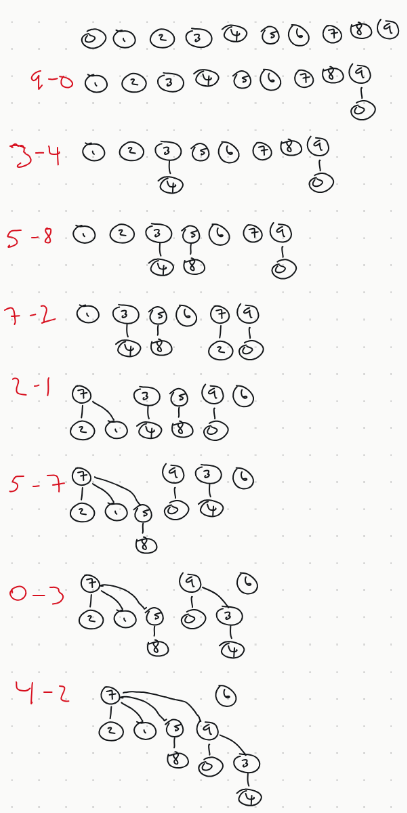
\includegraphics[width=0.5\textwidth]{exercise-03-weighted-quick-union-forest-of-trees}
			\caption{Forest of trees representation of \texttt{id[]} for quick-union in Exercise 2.}
			\label{ex-03}
		\end{figure}
		See Figure~\ref{ex-03}.
	\end{sol}
	\begin{ex}{4}
		Show the contents of the \texttt{sz[]} and \texttt{id[]} arrays and the number of array
		accesses for each input pair corresponding to the weighted quick-union examples in the
		text (both the reference input and the worst-case input).
	\end{ex}
	\begin{sol}
		First the reference input:
		\begin{center}
			\begin{tabular}{cc|cccccccccc|c|cccccccccc}
				\multicolumn{23}{c}{Weighted Quick-Union, Reference Input}\\
				{} & {} & \multicolumn{11}{c}{\texttt{id[]}} & \multicolumn{10}{c}{\texttt{sz[]}}\\
				\texttt{p} & \texttt{q} & 0 & 1 & 2 & 3 & 4 & 5 & 6 & 7 & 8 & 9 & \texttt{id[]} Accesses
				& 0 & 1 & 2 & 3 & 4 & 5 & 6 & 7 & 8 & 9\\
				\hline
				4  & 3  & 0 & 1 & 2 & {\color{green} 3} & {\color{green}4} & 5 & 6 & 7 & 8 & 9 & {} &
				1 & 1 & 1 & 1 & 1 & 1 & 1 & 1 & 1 & 1\\
				{} & {} & 0 & 1 & 2 & {\color{red}4} & 4 & 5 & 6 & 7 & 8 & 9 & 3 &
				1 & 1 & 1 & 1 & 2 & 1 & 1 & 1 & 1 & 1\\
				
				3  & 8  & 0 & 1 & 2 & {\color{green}4} & {\color{green}4} & 5 & 6 & 7 & {\color{green}8} & 9 & {}
				\\
				{} & {} & 0 & 1 & 2 & 4 & 4 & 5 & 6 & 7 & {\color{red}4} & 9 & 5
				& 1 & 1 & 1 & 1 & 3 & 1 & 1& 1  & 1 & 1\\
				
				6  & 5  & 0 & 1 & 2 & 4 & 4 & {\color{green}5} & {\color{green}6} & 7 & 4 & 9 & {}
				\\
				{} & {} & 0 & 1 & 2 & 4 & 4 & {\color{red}6} & 6 & 7 & 4 & 9 & 3
				& 1 & 1 & 1 & 1 & 3 & 1 & 2& 1  & 1 & 1\\
				
				9  & 4  & 0 & 1 & 2 & {\color{green}4} & {\color{green}4} & 6 & 6 & 7 & {\color{green}4} & {\color{green}9} & {}
				\\
				{} & {} & 0 & 1 & 2 & 4 & 4 & 6 & 6 & 7 & 4 & {\color{red}4} & 3
				& 1 & 1 & 1 & 1 & 4 & 1 & 2& 1  & 1 & 1\\
				
				2  & 1  & 0 & {\color{green}1} & {\color{green}2} & 4 & 4 & 6 & 6 & 7 & 4 & 4 & {}
				\\
				{} & {} & 0 & {\color{red}2}   & 2 & 4 & 4 & 6 & 6 & 7 & 4 & 4 & 3
				& 1 & 1 & 2 & 1 & 4 & 1 & 2& 1  & 1 & 1\\
				
				8  & 9  & 0 & 2  & 2 & 4 & 4 & 6 & 6 & 7 & 4 & 4 & {}\\
				{} & {} & 0 & 2  & 2 & 4 & 4 & 6 & 6 & 7 & 4 & 4 & 6
				\\
				
				5  & 0  & {\color{green}0} & 2  & 2 & 4 & 4 & {\color{green}6} & {\color{green}6} & 7 & 4 & 4 & {}\\
				{} & {} & {\color{red}6} & 2  & 2 & 4 & 4 & 6 & 6 & 7 & 4 & 4 & 5
				& 1 & 1 & 2 & 1 & 4 & 1 & 3& 1  & 1 & 1\\
				
				7  & 2  & 6 & {\color{green}2}  & {\color{green}2} & 4 & 4 & 6 & 6 & {\color{green}7} & 4 & 4 & {}\\
				{} & {} & 6 & 2  & 2 & 4 & 4 & 6 & 6 & {\color{red}2} & 4 & 4 & 3
				& 1 & 1 & 3 & 1 & 4 & 1 & 3& 1  & 1 & 1\\
				
				6  & 1  & 6 & {\color{green}2}  & 2 & 4 & 4 & 6 & {\color{green}6} & 2 & 4 & 4 & {}\\
				{} & {} & 6 & {\color{green}6}  & 2 & 4 & 4 & 6 & 6 & 2 & 4 & 4 & 5
				& 1 & 1 & 3 & 1 & 4 & 1 & 6& 1  & 1 & 1\\
				
				1  & 0  & 6 & 6  & 2 & 4 & 4 & 6 & 6 & 2 & 4 & 4 & {}\\
				{} & {} & 6 & 6  & 2 & 4 & 4 & 6 & 6 & 2 & 4 & 4 & 8\\
				
				6  & 7  & 6 & 6  & 2 & 4 & 4 & 6 & 6 & 2 & 4 & 4 & {}\\
				{} & {} & 6 & 6  & 2 & 4 & 4 & 6 & 6 & 2 & 4 & 4 & 6\\
			\end{tabular}
		\end{center}
		Next, the worst-case input:
		\begin{center}
			\begin{tabular}{cc|cccccccc|c|cccccccc}
								\multicolumn{19}{c}{Weighted Quick-Union, Worst-Case Input}\\
				{} & {} & \multicolumn{9}{c}{\texttt{id[]}} & \multicolumn{8}{c}{\texttt{sz[]}}\\
				\texttt{p} & \texttt{q} & 0 & 1 & 2 & 3 & 4 & 5 & 6 & 7 & \texttt{id[]} Accesses
				& 0 & 1 & 2 & 3 & 4 & 5 & 6 & 7\\
				\hline
				0  & 1  & {\color{green}0} & {\color{green}1} & 2 & 3 & 4 & 5 & 6 & 7 & {}
				& 1 & 1 & 1 & 1 & 1 & 1 & 1 & 1\\
				{} & {} & 0 & {\color{red}0} & 2 & 3 & 4 & 5 & 6 & 7 & 3
				& 2 & 1 & 1 & 1 & 1 & 1 & 1 & 1\\
				
				2  & 3  & 0 & 0 & {\color{green}2} & {\color{green}3} & 4 & 5 & 6 & 7 & {}\\
				{} & {} & 0 & 1 & 2 & {\color{red}2} & 4 & 5 & 6 & 7 & 3
				& 2 & 1 & 2 & 1 & 1 & 1 & 1 & 1\\
				
				4  & 5  & 0 & 0 & 2 & 2 & {\color{green}4} & {\color{green}5} & 6 & 7 & {}\\
				{} & {} & 0 & 1 & 2 & 2 & 4 & {\color{red}4} & 6 & 7 & 3
				& 2 & 1 & 2 & 1 & 2 & 1 & 1 & 1\\
				
				6 & 7 & 0 & 0 & 2 & 2 & 4 & 4 & {\color{green}6} & {\color{green}7} & {}\\
				{} & {} & 0 & 1 & 2 & 2 & 4 & 4 & 6 & {\color{red}6} & 3
				& 2 & 1 & 2 & 1 & 2 & 1 & 2 & 1\\
				
				0  & 2  & {\color{green}0} & 0 & {\color{green}2} & 2 & 4 & 4 & 6 & 6 & {}\\
				{} & {} & 0 & 0 & {\color{red}0} & 2 & 4 & 4 & 6 & 6 & 3
				& 4 & 1 & 2 & 1 & 2 & 1 & 2 & 1\\
				
				4  & 6  & 0 & 0 & 0 & 2 & {\color{green}4} & 4 & {\color{green}6} & 6 & {}\\
				{} & {} & 0 & 0 & 0 & 2 & 4 & 4 & {\color{red}4} & 6 & 3
				& 4 & 1 & 2 & 1 & 4 & 1 & 2 & 1\\
				
				0  & 4  & {\color{green}0} & 0 & 0 & 2 & {\color{green}4} & 4 & 4 & 6 & {}\\
				{} & {} & 0 & 0 & 0 & 2 & {\color{red}0} & 4 & 4 & 6 & 3
				& 8 & 1 & 2 & 1 & 4 & 1 & 2 & 1\\
			\end{tabular}
		\end{center}
	\end{sol}
	\begin{ex}{5}
		Estimate the minimum amount of time (in days) that would be required for quick-find
		to solve a dynamic connectivity problem with $10^9$ sites and $10^6$ input pairs,
		on a computer capable of executing $10^9$ instructions per second. Assume that each
		iteration of the  inner \texttt{for} loop requires 10 machine instructions.
	\end{ex}
	\begin{sol}
		Because there are $10^6$ input pairs, that means the program requires $10^6$ iterations,
		regardless of the union-find implementation. Let $n=10^9$. The inner loop of quick-find
		is a \texttt{for} loop that iterates through all $n=10^9$ sites. By assumption, each
		iteration takes 10 machine instructions, so the cost of the inner for loop is
		$10^{10}$ instructions. Altogether, we need $10^6\cdot 10^{10}=10^{16}$ instructions
		in order to process all input pairs. With a computer capable of executing $10^9$
		instructions per second, it would take $10^{16}/10^9=10^7$ seconds to process all pairs.
		Now the total time $T$ would be:
		\begin{align*}
			T \approx 10^7\text {seconds} \cdot \frac{1 \text{ day}}{86400 \text{ seconds}} \approx 116 \text{ days}
		\end{align*}
	\end{sol}
	\begin{ex}{6}
		Repeat Exercise 1.5.5 for weighed quick union.
	\end{ex}
	\begin{sol}
		A similar analysis holds. That is, we require $10^6$ iterations to process all $10^6$
		pairs. We still have $n=10^9$. However, the order of growth is $\lg n\approx 23$. Assuming
		the rest of the information is the same:
		\begin{align*}
			T & \approx \frac{10^6\cdot \lg (10^9) \cdot 10 \text{ instructions}}{10^9 \text{ instructions per sec}}\\
			&=\frac{\lg(10^9)\text{ seconds}}{10^2}\\
			&\approx 0.3 \text{ seconds}
		\end{align*}
	\end{sol}
	\begin{ex}{7}
		Develop classes \texttt{QuickUnionUF} and \texttt{QuickFindUF} that implement quick-union
		and quick-find, respectively.
	\end{ex}
	\begin{sol}
		See the \texttt{com.segarciat.algs.ch1.sec5.ex07} package.
	\end{sol}
	\begin{ex}{8}
		Give a counterexample to show why this intuitive implementation of \texttt{union()}
		for quick-find is not correct:
		\begin{lstlisting}
	public void union(int p, int q)
	{
		if (id[p] == id[q]) return;
		
		// Rename p's component to q's name.
		for (int i = 0; i < id.length; i++)
			if (id[i] == id[p]) id[i] = id[q];
		count--;
	}
		\end{lstlisting}
	\end{ex}
	\begin{sol}
		Suppose we have three sites, numbered 0, 1, 2, and we get the following input sequence:
		\begin{lstlisting}[language={}]
0-1
0-2
		\end{lstlisting}
		The end result is that all sites will be connected and there will only be one component
		at the end. However, the contents of the \texttt{id[]} array are as follows after
		the algorithm above is applied:
		\begin{lstlisting}[language={}]
# start
0 1 2

# after 0-1
1 1 2

# after 0-2
2 1 2
		\end{lstlisting}
		The problem surfaces while processing input pair \texttt{0-2}. The algorithm determines
		that the identifiers of the components are distinct, so it proceeds to rename
		\texttt{p}'s component to \texttt{q}'s component. In this case, renaming \texttt{0}'s
		component (with identifier 1) to \texttt{2}'s component (with identifier 2). The
		first iteration changes \texttt{id[0]} to \texttt{2}, which is correct. In the second
		iteration, \texttt{id[1]} is compared against \texttt{id[0]}, and they are determined
		to be unequal because \texttt{id[0]} was changed in the previous iteration to \texttt{2}.
		Thus, \texttt{id[1]} will remain as \texttt{1}, which is incorrect.
	\end{sol}
	\begin{ex}{9}
		Draw the tree corresponding to the \texttt{id[]} array depicted at right. Can this
		be the result of running weighted quick-union? Explain why this is impossible or give a
		sequence of operations that results in this array.
		\begin{center}
			\begin{tabular}{c|cccccccccc}
				\texttt{i} & 0 & 1 & 2 & 3 & 4 & 5 & 6 & 7 & 8 & 9\\
				\hline
				\texttt{id[i]} & 1 & 1 & 3 & 1 & 5 &6 & 1 & 3 & 4 & 5
			\end{tabular}
		\end{center}
	\end{ex}
	\begin{sol}
		\begin{figure}
			\centering
			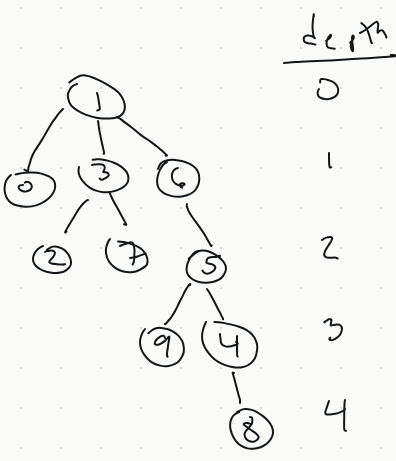
\includegraphics[width=0.5\textwidth]{exercise-10-union-find-tree}
			\caption{Tree from array in Exercise 10.}
			\label{ex-10}
		\end{figure}
		See Figure~\ref{ex-10}. The tree has $10$ nodes, and its height is $4$. By Proposition H
		in \cite{sedgewick_wayne}, the depth of any node in a forest built by weighted quick-union
		of $n$ sites is at most $\lg n$. Letting $n=10$, we see that $\lg n<4$. Therefore,
		it's impossible for weighted quick union to have produced such an array.
	\end{sol}
	\begin{ex}{10}
		In the weighted quick-union algorithm, suppose that we set \texttt{id[find(p)]} to
		\texttt{q} instead of to \texttt{id[find(q)]}. Would the resulting algorithm be
		correct?
	\end{ex}
	\begin{sol}
		Yes because it would ensure that \texttt{p} and \texttt{q} are on the same tree
		and hence the same component. However, \texttt{q} may not be the root of the tree;
		it may be a leaf or a non-root internal node. As a result, we would not have the
		logarithmic performance guarantee of weighted quick union.
	\end{sol}
	\begin{ex}{11}
		Implemented \emph{weighted quick-find}, where you always change the \texttt{id[]}
		entries of the smaller component to the identifier of the larger component.
		How does this affect performance?
	\end{ex}
	\begin{sol}
		This is not an improvement over (unweighted) quick-find. In particular, if \texttt{p} is any
		site in any component, then \texttt{id[p]} always evaluates to the identifier of
		the root of the tree. As a result, \texttt{find()} takes constant time. However,
		in order to change the \texttt{id[]} entries in the smaller component to the
		identifier of the larger component in the \texttt{union()} implementation, we must
		iterate through all the sites. This is necessary because the links are
		unidirectional; that is, they always point towards the root. In particular,
		if an input pair consists of two roots, the current arrangement does not
		provide an easy way to find the leaves, or any of the internal non-root
		nodes. As a result, the performance of \texttt{union()} degrades to linear,
		as it was in the (unweighted) quick-find implementation. In this case,
		maintaining the size of the trees for each component in the \texttt{sz[]} array
		added complexity to our algorithm and increased our space requirement,
		with no payoff.
	\end{sol}
	\begin{ex}{12}
		\emph{Quick-union with path compression}. Modify quick-union (page 224) to include
		\emph{path compression}, by adding a loop to \texttt{find()} that links every site
		on the path from \texttt{p} to the root. Give a sequence of input pairs that causes
		this method to produce a path of length 4. \emph{Note}: The amortized cost per
		operation for this algorithm is known to be logarithmic.
	\end{ex}
	\begin{sol}
		See the \texttt{com.segarciat.algs4.ch1.sec5.ex12.QuickUnionPC} class. The following
		sequence of input pairs yields a path of length 4:
		\begin{lstlisting}[language={}]
1-0 2-3 0-2 0-4 4-5
		\end{lstlisting}
		In general, joining the root of a tree with another will increase the tree height.
		This is because if \texttt{p} is a root, then \texttt{find(p)} will only encounter
		\texttt{p} on the path to the root. Thus, the paths with greater depth will not
		be renamed. In the tree that is formed, node \texttt{3} has a depth of 4.
	\end{sol}
	\begin{ex}{13}
		\emph{Weighted quick-union with path compression}. Modify weighted quick-union (Algorithm 1.5)
		to implement path compression, as described in Exercise 1.5.12. Give a sequence of input
		pairs that causes this method to produce a tree of height 4.
		\emph{Note}: The amortized cost per operation for this algorithm is known to be bounded by
		a function known as the \emph{inverse Ackermann function} and is less than 5 for any conceivable
		value of $n$ that arises in practice.
	\end{ex}
	\begin{sol}
		The following sequence of input pairs produces a tree of height 3 with \texttt{0} as the root:
		\begin{lstlisting}[language={}]
0-1 2-3 0-2 4-5 6-7 0-4
		\end{lstlisting}
		The following sequence of input pairs produces another tree of height 3 with \texttt{8} as the root:
		\begin{lstlisting}[language={}]
8-9 10-11 8-10 12-13 14-15 8-12
		\end{lstlisting}
		Finally, the following pair combines the trees and creates a tree of height 4 rooted at \texttt{0}:
		\begin{lstlisting}[language={}]
0-8
		\end{lstlisting}	
		In this tree, there are two nodes with a depth of 4: node \texttt{7} and node \texttt{15}.
	\end{sol}
	\begin{ex}{14}
		\emph{Weighted quick-union by height}. Develop a \texttt{UF} implementation that uses the
		same basic strategy as weighted quick-union but keeps track of tree height and always
		links the shorter tree to the taller one. Prove a logarithmic upper bound on the height
		of the trees for $n$ sites with your algorithm.
	\end{ex}
	\begin{sol}
		I claim when the size of every tree of $n$ sites is at most $\lg n$. The proof is
		by strong induction.
		\begin{proof}
			If $n=1$, then $\lg 1=0$, proving the base case. Suppose that $n>1$, and whenever a tree
			is built out of $k<n$ sites, then its height is at most $\lg k$. If the algorithm
			has more than 1 component, then each tree has less than $n$ sites, and hence, the
			result follows by the inductive hypothesis. Suppose, however, that there is
			only one component, and hence there is a single tree with $n$ sites.
			
			Let  $n_1$ and $n_2$ be the number of sites in the two trees prior to the input pair
			that causes them to combine into one tree. If the two trees have different heights,
			then the algorithm does not increment the height of the resulting tree when the
			smaller one is attached to the larger one, and the result holds since in this
			case the height is less than $\max\{\lg(n_1), \lg(n_2)\}\leq \lg(n)$. If the
			trees have different heights, then the algorithm increases the height by $1$.
			Since the height of each tree is bounded by $\lg(n_1)$ and $\lg(n_2)$, respectively,
			and the heights are the same, this means that both of these serve as upper bounds.
			Thus, if we let $N=\min\{n_1,n_2\}$, then the height of the resulting tree
			is bounded by $1 + \lg(N)$, and hence
			\begin{align*}
				\text{height}& \leq 1 + \lg (N)\\
				 &=\lg(2) + \lg(N)\\
				 &=\lg(2N)\\
				 &=\lg (N + N)\\
				 &\leq \lg(n_1 + n_2)\\
				 &=\lg(n)
			\end{align*}
			The result now holds for induction.
		\end{proof}
	\end{sol}
	\begin{ex}{15}
		\emph{Binomial trees}. Show that the number of nodes at each level in the worst-case
		trees for weighted quick-union are \emph{binomial coefficients}. Compute the average
		depth of a node in a worst-case tree with $k=2^n$ nodes.
	\end{ex}
	\begin{sol}
		Note that the level of a node is one more than the depth.
		
		\begin{proof}
			I will prove that if $T$ is a tree of height $h$ built by the worst-case input,
			then level $k$ is $\binom{h}{k-1}$, where $0\leq k-1\leq h$ and $h$ is an integer.
			
			If there are two nodes, then the height of the tree is $h=1$, 
			and the tree has $\binom{h}{1-1}=\binom{1}{0}=1$ node at level $1$, and
			$\binom{h}{2-1}=\binom{1}{1}$ nod at level $2$. Thus the base case holds.
			
			Proceeding by induction, suppose that the algorithm has continued to process
			worst-case input and that the height of every tree of height $m < h$
			has the property that level $k$ has $\binom{m}{k-1}$ nodes, where $h>1$
			and $0\leq k-1\leq m$. Under the assumption of worst-case input, the algorithm
			will only combine two trees that of the same size.
			
			Suppose $T_1$ and $T_2$ are two trees of height $m$ that are combined into a tree
			$T$ of height $h$. Note that $m + 1=h$
			Without loss of generality, suppose that $T_2$ is joined to $T_1$.
			Then the root of $T$ is the root of $T_1$, and the nodes in $T_1$ retain
			their level in the new tree $T$. However, a node at level $i$ in $T_2$
			moves to level $k+1$ in $T$ when $T_2$ is joined to $T_1$. As a result,
			the number of nodes at level $k$ in $T$ is given by:
			\begin{align*}
				\text{ \# of nodes at level $k$} = \binom{m}{k-1} + \binom{m}{(k-1) -1},\quad 1\leq k-1\leq m
			\end{align*}
			for all levels $k$ greater than $1$ (not the root). The first term is
			the number of nodes at level $k$ as a result of $T_1$, whose place in the
			resulting tree $T^*$ is unchanged because $T_2$ is joined to $T_1$.
			The second term follows from the fact that every node in $T_2$ has moved
			down a level.
			
			Pascal's triangle says that
			\begin{align*}
				\binom{h}{k-1}=\binom{m+1}{k-1} = \binom{m}{k-1}+\binom{m}{(k-1)-1},\quad 1\leq k-1\leq m
			\end{align*}
			The resulting formula can be extended to $0\leq k-1\leq m+1$ because at level
			$1$ we only have the root of $T_1$, so we have $\binom{h}{1-1}=\binom{m+1}{0}=1$,
			and at level $h+1$ we only have the single node that is at level $m$ in tree $T_2$,
			consistent with $\binom{h}{(h+1)-1}=\binom{h}{h}=1$.
		\end{proof}
		
		If a worst-case tree has $k=2^n$ nodes, then the height of such a tree is $\lg(k)=\lg(2^n)=n$,
		so the average depth of any node is
		\begin{align*}
			\frac{\sum_{j=0}^{n}\binom{n}{j}\cdot j}{2^n} = \frac{n\cdot 2^{n-1}}{n}=\frac{n}{2}
		\end{align*}
		where I have used the formula $\sum_{j=0}^{n}\binom{n}{j}\cdot j=n\cdot 2^{n-1}$;
		see \href{https://math.stackexchange.com/a/123665}{Pedro's proof on StackExchange}.
	\end{sol}
	\begin{ex}{16}
		\emph{Amortized cost plots}. Instrument your implementations from Exercise 1.5.7
		to make amortized cost plots like those in the text.
	\end{ex}
	\begin{sol}
		See the classes in the \texttt{com.segarciat.algs4.ch1.sec5.ex16} package.
	\end{sol}
	\begin{ex}{17}
		\emph{Random connections}. Develop a \texttt{UF} client \texttt{ErdosRenyi} that
		takes an  integer value \texttt{n} from the command line, generates random pairs of
		integers between \texttt{0} and \texttt{n-1}, calling \texttt{connected()} to
		determine if they are connected and then \texttt{union()} if not (as in our
		development client), looping until all sites are connected, and printing the number
		of connections generated. Package your program as a static method \texttt{count()}
		that takes \texttt{n} as an argument and returns the number of connections and
		a \texttt{main()} that takes \texttt{n} from the command line, calls \texttt{count},
		and prints the returned value.
	\end{ex}
	\pagebreak
	\printbibliography
\end{document}